\documentclass{article}%
\usepackage{amsmath}%
\usepackage{amsfonts}%
\usepackage{amssymb}%
\usepackage{graphicx}
\usepackage{hyperref}

%-------------------------------------------
\newtheorem{theorem}{Theorem}
\newtheorem{acknowledgement}[theorem]{Acknowledgement}
\newtheorem{algorithm}[theorem]{Algorithm}
\newtheorem{axiom}[theorem]{Axiom}
\newtheorem{case}[theorem]{Case}
\newtheorem{claim}[theorem]{Claim}
\newtheorem{conclusion}[theorem]{Conclusion}
\newtheorem{condition}[theorem]{Condition}
\newtheorem{conjecture}[theorem]{Conjecture}
\newtheorem{corollary}[theorem]{Corollary}
\newtheorem{criterion}[theorem]{Criterion}
\newtheorem{definition}[theorem]{Definition}
\newtheorem{example}[theorem]{Example}
\newtheorem{exercise}[theorem]{Exercise}
\newtheorem{lemma}[theorem]{Lemma}
\newtheorem{notation}[theorem]{Notation}
\newtheorem{problem}[theorem]{Problem}
\newtheorem{proposition}[theorem]{Proposition}
\newtheorem{remark}[theorem]{Remark}
\newtheorem{solution}[theorem]{Solution}
\newtheorem{summary}[theorem]{Summary}
\newenvironment{proof}[1][Proof]{\textbf{#1.} }{\ \rule{0.5em}{0.5em}}
\setlength{\textwidth}{7.0in}
\setlength{\oddsidemargin}{-0.35in}
\setlength{\topmargin}{-0.5in}
\setlength{\textheight}{9.0in}
\setlength{\parindent}{0.3in}
\begin{document}

\begin{flushright}
\textbf{Dylan Bonsell \\
Feb. 10, 2014}
\end{flushright}

\begin{center}
\textbf{CS 322 Assignment 3 \\
Writeup} \\
\end{center}

\section*{Overview:}
The findings in this assignment were insightful, and show a lot about how much messaging and the methods used can affect program run times and efficiency.
The programs in this wrieup were run on a intel i7 clocked at 4.9GHz, 16GB DDR3 2133mhz ram, running on an ssd for increased program load time. 

\section*{Compilation}
I used a very basic form of compilation, as described below:
\begin{enumerate}
\item To compile, I used: mpicc part.c -o part
\item To run, I used: mpirun -np \#processes ./part
\end{enumerate}

\section*{Analysis}
The way I analized run times is with $MPI\_Wtime$, from the start of the program to the end, to measure in seconds. 
Then, I took values for 10 iterations for np = 2, 8, 16, 32 and 1000 iterations and 10,000 iterations in the loop.

Each data value is run on a system at rest, I.E. no other tasks running.
\begin{enumerate}
\item 1000 Loop Iterations

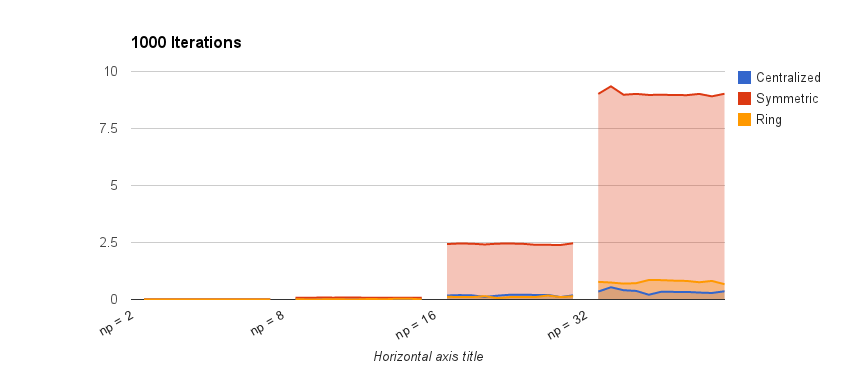
\includegraphics[scale=0.5]{chart_1.png}

These findings are interesting, but not surprising - Centralized is the most efficient, then Ring, and the worst by far is Symmetric. 
Centralized is just barely more efficient than Ring because ring requires each processor to send and recieve to 2 processes, whereas all processors that aren't
0 send and recieve to only 1 process in Centralized. 
Symmetric is, by far, exponantially worse, because it requires so many messages to be passed, for each processor, so it is not surprising that it is exponenitally worse.
\vspace{20mm}
\item 10,000 Loop Iterations

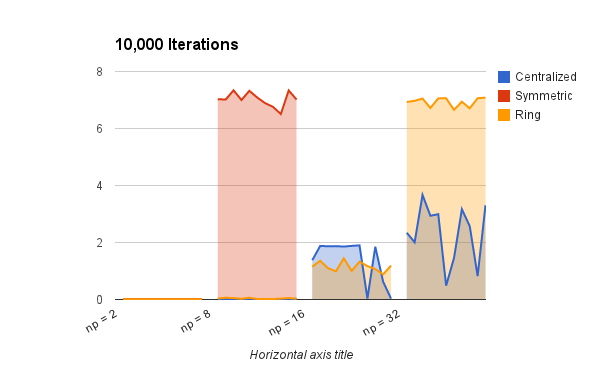
\includegraphics[scale=0.7]{chart_2.png}

For this one, I ran into memory issues at $np >= 16$ for Symmetric, because of overflow errors.
Other that that, the analysis is the same as before, except for some small deviations at $np = 16$, to which I accounted for by making the first value an average of all ten values. I believe these outliers to be time specific, perhaps the system had another high-intensity task running. 
\end{enumerate}

\section*{Sources}
All of my data can be found on my Google Drive, with the following link:
\vspace{10mm}

\href{https://docs.google.com/spreadsheet/ccc?key=0AtGVZx-NN2eVdEFtdGFROGFaSDQ3bVVVb2dwWmpOdGc&usp=sharing}{Assignment 3 Analysis Data}



\end{document}